\documentclass[a4paper,11pt]{article}
\usepackage[utf8]{inputenc}
\usepackage{algorithmic}
\usepackage{algorithm}
\usepackage{pst-plot}
\usepackage{graphicx}
\usepackage{endnotes}
\usepackage{graphics}
\usepackage{floatflt}
\usepackage{wrapfig}
\usepackage{amsfonts}
\usepackage{amsmath}
\usepackage{verbatim}
\usepackage{hyperref}
\usepackage{multirow}
\usepackage{pdflscape}

\usepackage{hyperref}
\hypersetup{pdfborder={0 0 0 0}}

\pdfpagewidth 210mm
\pdfpageheight 297mm 
\setlength\topmargin{0mm}
\setlength\headheight{0mm}
\setlength\headsep{0mm}
\setlength\textheight{250mm}	
\setlength\textwidth{159.2mm}
\setlength\oddsidemargin{0mm}
\setlength\evensidemargin{0mm}
\setlength\parindent{7mm}
\setlength\parskip{0mm}

\newenvironment{exercise}[3]{\paragraph{Exercise #1: #2 (#3pt)}\ \\}{
\medskip}
\newcommand{\question}[2]{\setlength\parindent{0mm}\ \\$\mathbf{Q_#1:}$ #2\ \\}

\author{\large{Ilya Kuzovkin, Raul Vicente}}
\title{\huge{Introduction to Computational Neuroscience}\\\LARGE{Practice III: Data Analysis - Spiking Data}}

\begin{document}
\maketitle

Last time we had a look at continuous brain data: strength of EEG signal was changing over time. Another very popular form of data, mostly associated with single neuron recordings, is \emph{spiking} data. Concept is very simple: we attach a sensor to the neuron and when neuron fires we write "1" into our data file, otherwise we write "0". The resulting data shows us for each time point whether neuron has fired or not.

\begin{exercise}{1}{Raster plot}{0.5}
Let us start by plotting some spiking data. Under the \texttt{data/lgn} folder you have recordings from 72 neurons of a mouse. \texttt{Matlab/Octave} users can use files in the \texttt{matlab} folder, the same data is available in the plain text format in the \texttt{plain} folder.

Dataset has spiking data recorded while the mouse was presented with a stimulus: moving bar which has different orientations. On Figure \ref{fig:lgnstimulus} you can see an example: spiking pattern of one particular neuron seem to indicate that this 
neuron is more active when the bar is tilted 45 degrees clockwise from the horizontal position. And it's activity fades when bar changes the orientation. Our dataset was created while conducting the similar experiment. We would like to rediscover from that data, than indeed different neurons respond to different orientations.
\begin{figure}[H]
   \centering
   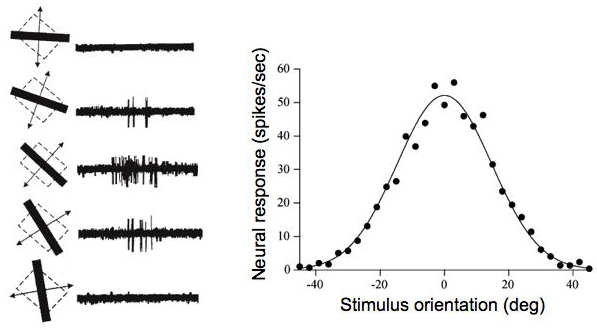
\includegraphics[width=0.8\textwidth]{orientation.jpg} 
   \caption{Neuronal response to different orientations of the bar.}
   \label{fig:lgnstimulus}
\end{figure}

\texttt{Matlab} files have names \texttt{mlgnori\_NN.mat} where \texttt{NN} is the number of the neuron. When you load it to you environment you will find that each file has a structure with two elements: \texttt{spktimes} and \texttt{stim}. The first one is $M\times N \times T$ matrix where $M$ is the stimulus number, $N$ is the repeat number at $T$ is time in milliseconds. The second one describes the stimulus, open it and you will see what information is there.

Plain files with spiking data have names \texttt{neuron\_NN\_stimulus\_SS.csv} where \texttt{NN} is the number of the neuron and \texttt{SS} is the number of the stimulus. Inside each file one line represents one trial. For each millisecond it has value 0 (no spike) or 1 (spike). Files with names \texttt{stimulus\_SS.csv} describe the stimulus: they hold four values:
\begin{enumerate}
\itemsep 0em
	\item Time before the stimulus (in seconds).
	\item Duration of the stimulus (in seconds).
	\item Time after the stimulus (in seconds).
	\item Orientation of the stimulus (in degrees).
\end{enumerate}
\end{exercise}
You task is to take any neuron and plot all trials as a raster plot (see Figure \ref{fig:raster_plot}).
\begin{figure}[H]
   \centering
   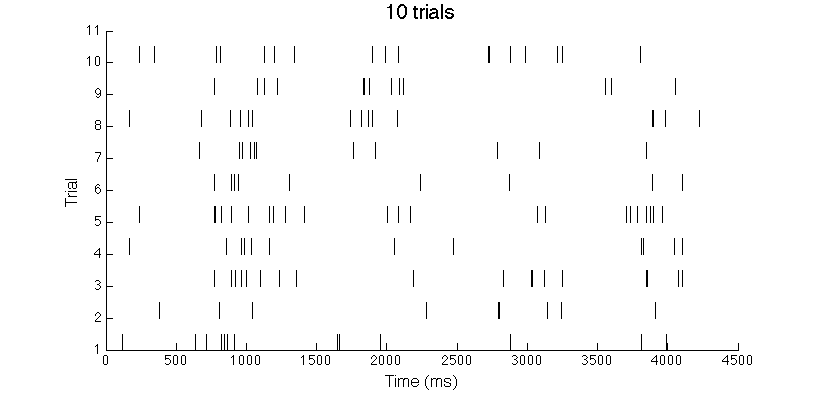
\includegraphics[width=0.7\textwidth]{raster10tr.png} 
   \caption{Raster plot of 10 trials on same neuron}
   \label{fig:raster_plot}
\end{figure}
On the $X$ axis we have time and on the $Y$ axis trials. A vertical bar indicates a spike. To draw a vertical line in \texttt{Matlab} you can use
\begin{verbatim}
	line([t t], [tr tr+0.5], 'Color', 'k');
\end{verbatim}
where \texttt{t} is time and \texttt{tr} is number of trial ($Y$ coordinate of a line more generally speaking).

\begin{exercise}{2}{More raster plots}{0.5}
The next step is to create two more raster plots. The first one will illustrate behaviour of all neurons under the same stimulus, while the other one will have responses of the same neuron but to the different stimuli.

First we need to average spiking data so that each neuron would be represented by one vector. Simplest way to do that is just to add trials together. If you have 10 trials, each of them is a vector of length 4500 time points, then just sum them together to obtain one vector of length 4500. After that replace all values which are grater than 1 with 1.

Create the following two plots:
\begin{enumerate}
	\item Raster plot, where on $Y$ axis we have all 72 neuron responses to the same stimulus (choose any). Please note that in our dataset different recordings have different length, this should not be a problem.
	\item Raster plot, where on $Y$ axis we have all 13 stimuli and responses from the same neuron (choose any) to those stimuli.
\end{enumerate}


\end{exercise}

\begin{exercise}{3}{Post-Stimulus Time Histogram (PSTH)}{0.5}
Another useful analysis tool is a histogram, where on $X$ axis we have time points (or time ranges) and on $Y$ axis number of spikes that occurred during given time range. It is called \emph{Post-Stimulus Time Histogram (PSTH)}.
\begin{enumerate}
	\item Choose any neuron, any stimulus.
	\item Take an average over all trials as we did before.
	\item Choose time window, for example 20ms or 50ms.
	\item Plot a histogram, where on the $X$ axis we have time windows and on the $Y$ axis the number of spikes during that time window.
\end{enumerate}
\end{exercise}


\begin{exercise}{4}{Real Science}{1}
Now you have a set of tools to analyse the spiking data:
\begin{itemize}
	\item Raster plot
	\item PSTH
	\item Average number of spikes per unit of time (rate)
\end{itemize}
Use those tools and for each of 13 stimuli try to identify one or more neuron(s), which are specific to the particular stimulus. Describe what you did and report your findings.
\end{exercise}


\begin{exercise}{5}{???}{0.5}
Discuss something
\end{exercise}



\ \\
\ \\
\ \\
\ \\
\ \\
Please submit a \texttt{pdf} report with answers to the questions and comments about your solutions. Also submit a code for the programming exercise(s). Pack those into \texttt{zip} archive and upload to the course web page.

\end{document}










